\documentclass[11pt,a4paper]{article}
\usepackage{../shared/luxcover}
\usepackage[utf8]{inputenc}
\usepackage[T1]{fontenc}
\usepackage{amsmath,amssymb,amsfonts,amsthm}
\usepackage{graphicx}
\usepackage{hyperref}
\usepackage{booktabs}
\usepackage{listings}
\usepackage{xcolor}
\usepackage{tikz}
\usepackage{float}
\usepackage{enumitem}
\usepackage{array}
\usepackage{tabularx}
\input{../shared/lstlang}
\usetikzlibrary{arrows.meta,positioning,shapes.geometric,fit,calc}

\hypersetup{colorlinks=true,linkcolor=black,citecolor=blue,urlcolor=blue}

\lstset{
  basicstyle=\ttfamily\scriptsize,
  breaklines=true,
  frame=single,
  numbers=left,
  numberstyle=\tiny\color{gray},
  showstringspaces=false,
}

\newtheorem{theorem}{Theorem}
\newtheorem{definition}{Definition}
\newtheorem{remark}{Remark}

\title{LP-9702: Z-Wing\\Hybrid Post-Quantum Secure Channel}

\author{
Zach Kelling\thanks{Corresponding author: zach@lux.network}\\
\textit{Lux Industries, Inc.}\\
\texttt{research@lux.network}
}

\date{}

\begin{document}

\luxcoverpage

\begin{abstract}
Z-Wing is a hybrid post-quantum secure channel for Lux node-to-node and
agent-to-agent communication. The key encapsulation mechanism is X-Wing
(ML-KEM-768 $+$ X25519) per \texttt{draft-connolly-cfrg-xwing-kem}, used
verbatim with the standard SHA3-256 combiner so that Z-Wing is wire-compatible
with any conformant X-Wing implementation. Identity binding is hybrid
Ed25519 $+$ ML-DSA-65 with both signatures committing to the same handshake
transcript. The handshake is one round trip; after completion the channel
exposes \texttt{net.Conn}, so any byte-stream protocol --- in particular the
ZAP wire format (\texttt{luxfi/api/zap}) --- runs unmodified above it.
Z-Wing supersedes LP-9701 (RNS hybrid-PQ link), which used a Lux-specific
HKDF combiner and inlined identity binding into the handshake construction.
LP-9702 collapses the two PQ surfaces in Lux today (LP-9701 in Go,
\texttt{zap-protocol} hybrid in Rust) onto a single canonical construction.
\end{abstract}

\tableofcontents
\newpage

\section{Motivation}

Two hybrid post-quantum constructions are deployed in Lux today.

\begin{enumerate}[leftmargin=*]
  \item \textbf{LP-9701 (RNS hybrid link, Go).} Implemented in
        \texttt{luxfi/node/network/dialer/rns\_link.go}. Combines X25519
        and ML-KEM-768 with an ad-hoc combiner: the ML-KEM contribution
        is derived deterministically from a sorted hash of both peers'
        ML-KEM ephemeral public keys (rather than a true KEM
        encapsulation), then mixed with the X25519 ECDH output via
        HKDF-SHA256 under Lux-specific labels
        (\texttt{RNS-HybridLink-v1}, \texttt{rns-hybrid-link-keys},
        \texttt{RNS-MLKEM-Hybrid-v1}). Identity binding (Ed25519 $+$ ML-DSA-65)
        is fused into the handshake messages.
  \item \textbf{\texttt{zap-protocol} hybrid (Rust).} Implemented in
        \texttt{zap/src/crypto.rs}. X25519 $+$ ML-KEM-768 with HKDF-SHA256
        under the Lux-specific label \texttt{ZAP-HYBRID-HANDSHAKE-v1}.
        Identity is layered separately by the application.
\end{enumerate}

Both constructions are sound but neither is the IETF X-Wing combiner
(\texttt{draft-connolly-cfrg-xwing-kem}), which uses SHA3-256 with a
fixed 6-byte label and a fixed input order. That makes cross-org and
cross-language interop a per-implementation matter rather than a
standards-conformant property.

LP-9702 collapses both onto a single canonical construction:
\begin{itemize}[leftmargin=*]
  \item KEM: X-Wing exactly as specified by the IETF draft.
  \item Identity: Ed25519 $+$ ML-DSA-65, both signing the handshake
        transcript hash.
  \item Layering: the channel is a \texttt{net.Conn}; any byte-stream
        protocol rides on top with no further specification.
\end{itemize}

\section{Architecture}

\subsection{Layering}

\begin{figure}[H]
\centering
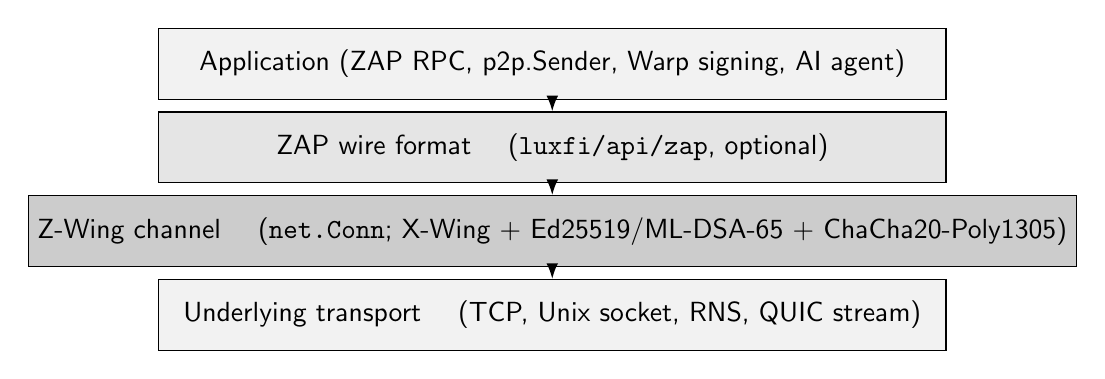
\begin{tikzpicture}[
    box/.style={draw, rectangle, minimum width=10cm, minimum height=0.9cm,
                font=\sffamily, align=center},
    arrow/.style={-{Latex[length=2mm]}, thick}
  ]
  \node[box, fill=black!5]  (app)   {Application (ZAP RPC, p2p.Sender, Warp signing, AI agent)};
  \node[box, fill=black!10, below=0.15cm of app] (zap)   {ZAP wire format \quad (\texttt{luxfi/api/zap}, optional)};
  \node[box, fill=black!20, below=0.15cm of zap] (zwing) {Z-Wing channel \quad (\texttt{net.Conn}; X-Wing $+$ Ed25519/ML-DSA-65 $+$ ChaCha20-Poly1305)};
  \node[box, fill=black!5,  below=0.15cm of zwing] (xport){Underlying transport \quad (TCP, Unix socket, RNS, QUIC stream)};

  \draw[arrow] (app)   -- (zap);
  \draw[arrow] (zap)   -- (zwing);
  \draw[arrow] (zwing) -- (xport);
\end{tikzpicture}
\caption{Z-Wing layering. The Z-Wing channel is a \texttt{net.Conn} whose
underlying byte stream is any reliable, ordered transport. ZAP and any
other application protocol ride above without modification.}
\label{fig:layering}
\end{figure}

\subsection{Components}

\begin{table}[H]
\centering
\begin{tabularx}{\textwidth}{lX}
\toprule
\textbf{Component} & \textbf{Construction} \\
\midrule
KEM        & X-Wing $=$ ML-KEM-768 (FIPS 203) $+$ X25519 (RFC 7748), combined with SHA3-256 \\
Identity   & Ed25519 (RFC 8032) $+$ ML-DSA-65 (FIPS 204), parallel signatures over transcript hash \\
KDF        & HKDF-SHA3-256 (RFC 5869 with FIPS 202 hash) \\
AEAD       & ChaCha20-Poly1305 (RFC 8439) \\
Transcript & SHA3-256 (FIPS 202) \\
\bottomrule
\end{tabularx}
\end{table}

\subsection{Channel interface}

The Z-Wing channel implements the Go \texttt{net.Conn} contract: \texttt{Read},
\texttt{Write}, \texttt{Close}, \texttt{LocalAddr}, \texttt{RemoteAddr}, the
three deadline setters. After \texttt{Handshake} returns, the channel is
authenticated, confidential, integrity-protected, and forward-secret.
\texttt{Read} and \texttt{Write} operate on plaintext bytes; encryption and
framing are handled internally.

\section{KEM Construction (Normative)}

\subsection{Component primitives}

\begin{table}[H]
\centering
\begin{tabularx}{\textwidth}{lll}
\toprule
\textbf{Quantity} & \textbf{Symbol} & \textbf{Size (bytes)} \\
\midrule
ML-KEM-768 encapsulation key   & $pk_M$ & 1184 \\
ML-KEM-768 decapsulation key   & $sk_M$ & 2400 \\
ML-KEM-768 ciphertext          & $ct_M$ & 1088 \\
ML-KEM-768 shared secret       & $ss_M$ & 32 \\
X25519 public key              & $pk_X$ & 32 \\
X25519 private key             & $sk_X$ & 32 \\
X25519 ephemeral public key (sender) & $ct_X$ & 32 \\
X25519 shared secret           & $ss_X$ & 32 \\
\midrule
X-Wing encapsulation key       & $pk$   & 1216 \\
X-Wing ciphertext              & $ct$   & 1120 \\
X-Wing shared secret           & $ss$   & 32 \\
\bottomrule
\end{tabularx}
\end{table}

The X-Wing encapsulation key is the byte concatenation $pk = pk_M \,\Vert\, pk_X$
(1184 $+$ 32 $=$ 1216 bytes). The X-Wing ciphertext is
$ct = ct_M \,\Vert\, ct_X$ (1088 $+$ 32 $=$ 1120 bytes).

\subsection{Combiner}

The X-Wing combiner is computed verbatim per
\texttt{draft-connolly-cfrg-xwing-kem}:

\begin{equation}
ss \;=\; \mathrm{SHA3\text{-}256}\!\left( ss_M \,\Vert\, ss_X \,\Vert\, ct_X \,\Vert\, pk_X \,\Vert\, L_{\mathrm{XW}} \right)
\label{eq:combiner}
\end{equation}

where the label $L_{\mathrm{XW}}$ is the 6-byte ASCII string
\texttt{\textbackslash./} concatenated with \texttt{/\textasciicircum\textbackslash}:

\begin{equation}
L_{\mathrm{XW}} \;=\; \texttt{0x5c}\;\texttt{0x2e}\;\texttt{0x2f}\;\texttt{0x2f}\;\texttt{0x5e}\;\texttt{0x5c}
\end{equation}

The label appears \emph{last} in the SHA3-256 input. The input order
$ss_M \Vert ss_X \Vert ct_X \Vert pk_X \Vert L_{\mathrm{XW}}$ is normative
and MUST NOT be permuted; the combiner is a fixed function of these five
operands in this exact order.

\subsection{Encapsulation}

Given peer encapsulation key $pk = pk_M \,\Vert\, pk_X$, the sender:

\begin{enumerate}[leftmargin=*]
  \item Generates an ephemeral X25519 key pair $(sk_X^e, pk_X^e)$ per RFC 7748,
        with the standard clamping of $sk_X^e$.
  \item Computes $ct_X \leftarrow pk_X^e$ and
        $ss_X \leftarrow \mathrm{X25519}(sk_X^e, pk_X)$. If $ss_X$ is the
        all-zero 32-byte string the sender MUST abort with a key-exchange
        failure (low-order point rejection per RFC 7748 \S6.1).
  \item Calls ML-KEM-768 encapsulation against $pk_M$, producing
        $(ct_M, ss_M)$ per FIPS 203.
  \item Computes $ss$ via Equation~\ref{eq:combiner}.
  \item Outputs $(ct, ss)$ where $ct = ct_M \,\Vert\, ct_X$.
\end{enumerate}

\subsection{Decapsulation}

Given decapsulation material $(sk_M, sk_X, pk_X)$ and ciphertext
$ct = ct_M \,\Vert\, ct_X$, the receiver:

\begin{enumerate}[leftmargin=*]
  \item Splits $ct$ into $ct_M$ (first 1088 bytes) and $ct_X$
        (next 32 bytes). Any other length MUST be rejected.
  \item Computes $ss_M \leftarrow \mathrm{ML\text{-}KEM\text{-}768.Decap}(sk_M, ct_M)$
        per FIPS 203. ML-KEM-768 implicit rejection is preserved: a
        malformed $ct_M$ yields a pseudorandom $ss_M$ and the protocol
        MUST proceed to the AEAD step, where the failure surfaces as
        an authentication-tag mismatch.
  \item Computes $ss_X \leftarrow \mathrm{X25519}(sk_X, ct_X)$. The
        all-zero output rejection of RFC 7748 \S6.1 MUST be enforced.
  \item Computes $ss$ via Equation~\ref{eq:combiner}.
\end{enumerate}

\section{Identity (Normative)}

\subsection{Hybrid identity}

A Z-Wing identity is the pair $(I_E, I_M)$ where $I_E$ is an Ed25519 key
pair (RFC 8032; 32-byte public key, 32-byte seed, 64-byte signature) and
$I_M$ is an ML-DSA-65 key pair (FIPS 204; 1952-byte public key,
4032-byte private key, 3309-byte signature).

The 32-byte node identifier is

\begin{equation}
\mathrm{NodeID} \;=\; \mathrm{SHA3\text{-}256}\!\left( I_E.\mathrm{pk} \,\Vert\, I_M.\mathrm{pk} \right) .
\end{equation}

\subsection{Canonical signing message}

Both identity signatures cover the same canonical message:

\begin{equation}
M_{\sigma} \;=\; \texttt{"zwing/1 transcript "} \,\Vert\, T
\end{equation}

where the literal prefix is the 19-byte ASCII string \texttt{"zwing/1
transcript "} (note the trailing space) and $T$ is the 32-byte
transcript hash defined in \S\ref{sec:handshake}.
The fixed prefix is a domain separator; signatures over $M_{\sigma}$
are not valid for any other Lux protocol context.

\subsection{Verification}

A peer's identity is bound to the channel only if BOTH signatures
verify against $M_{\sigma}$ under the advertised public keys. Either
signature failing aborts the handshake. Forging an accepted identity
binding requires breaking BOTH Ed25519 (current ECC attacks, including
quantum) AND ML-DSA-65 (lattice attacks).

\section{Handshake (Normative)}
\label{sec:handshake}

\subsection{Wire framing}

Handshake messages are length-prefixed: a 4-byte big-endian unsigned
length $L$ followed by $L$ bytes of payload. $L$ MUST NOT exceed
$2^{20}$ ($1\,048\,576$) bytes; receivers MUST close the underlying
transport on any larger value.

\subsection{HandshakeInit (initiator $\to$ responder)}

\begin{table}[H]
\centering
\begin{tabularx}{\textwidth}{llXr}
\toprule
\textbf{Field} & \textbf{Type} & \textbf{Description} & \textbf{Bytes} \\
\midrule
\texttt{magic}      & u32 BE & \texttt{0x5A57494E} (ASCII \texttt{"ZWIN"})       & 4 \\
\texttt{version}    & u8     & Protocol version, MUST be \texttt{0x01}            & 1 \\
\texttt{flags}      & u8     & Reserved, MUST be \texttt{0x00}                    & 1 \\
\texttt{ed25519\_pk}& bytes  & Initiator's long-term Ed25519 public key           & 32 \\
\texttt{mldsa\_pk}  & bytes  & Initiator's long-term ML-DSA-65 public key         & 1952 \\
\texttt{xwing\_pk}  & bytes  & Initiator's ephemeral X-Wing encapsulation key     & 1216 \\
\texttt{nonce\_i}   & bytes  & Initiator handshake nonce (uniformly random)       & 32 \\
\bottomrule
\end{tabularx}
\caption{HandshakeInit. Fixed total length: 3239 bytes. No padding, no extensions.}
\end{table}

\subsection{HandshakeResponse (responder $\to$ initiator)}

\begin{table}[H]
\centering
\begin{tabularx}{\textwidth}{llXr}
\toprule
\textbf{Field} & \textbf{Type} & \textbf{Description} & \textbf{Bytes} \\
\midrule
\texttt{magic}      & u32 BE & \texttt{0x5A57494E}                                & 4 \\
\texttt{version}    & u8     & MUST equal initiator's version                     & 1 \\
\texttt{flags}      & u8     & Reserved, MUST be \texttt{0x00}                    & 1 \\
\texttt{ed25519\_pk}& bytes  & Responder's long-term Ed25519 public key           & 32 \\
\texttt{mldsa\_pk}  & bytes  & Responder's long-term ML-DSA-65 public key         & 1952 \\
\texttt{xwing\_ct}  & bytes  & X-Wing ciphertext encapsulated to initiator's key  & 1120 \\
\texttt{nonce\_r}   & bytes  & Responder handshake nonce                          & 32 \\
\texttt{ed25519\_sig}& bytes & Responder's Ed25519 signature over $M_{\sigma}$    & 64 \\
\texttt{mldsa\_sig} & bytes  & Responder's ML-DSA-65 signature over $M_{\sigma}$  & 3309 \\
\bottomrule
\end{tabularx}
\caption{HandshakeResponse. Fixed total length: 6515 bytes.}
\end{table}

\subsection{HandshakeFinish (initiator $\to$ responder, encrypted)}

After deriving session keys, the initiator sends a single AEAD-protected
frame (per \S\ref{sec:transport}) carrying:

\begin{table}[H]
\centering
\begin{tabularx}{\textwidth}{llXr}
\toprule
\textbf{Field} & \textbf{Type} & \textbf{Description} & \textbf{Bytes} \\
\midrule
\texttt{ed25519\_sig}& bytes & Initiator's Ed25519 signature over $M_{\sigma}$    & 64 \\
\texttt{mldsa\_sig} & bytes  & Initiator's ML-DSA-65 signature over $M_{\sigma}$  & 3309 \\
\bottomrule
\end{tabularx}
\caption{HandshakeFinish (plaintext fields). Encrypted as the first
i$\to$r data frame.}
\end{table}

\begin{remark}
Z-Wing is therefore one round trip on the wire: HandshakeInit and
HandshakeResponse cross before any application data flows. The initiator's
signature is delivered as the first AEAD frame, encrypted under the
freshly derived session keys. This design preserves 1-RTT
(application data MAY be appended to the same TCP segment as
HandshakeFinish) while keeping the initiator identity hidden from
passive observers.
\end{remark}

\subsection{Transcript}

The transcript hash $T$ binds every byte either party put on the wire
during the handshake:

\begin{equation}
T \;=\; \mathrm{SHA3\text{-}256}\!\left( \texttt{HandshakeInit} \,\Vert\, \texttt{HandshakeResponseHeader} \right)
\end{equation}

where \texttt{HandshakeResponseHeader} is the responder's message with
\texttt{ed25519\_sig} and \texttt{mldsa\_sig} omitted (the first
$4 + 1 + 1 + 32 + 1952 + 1120 + 32 = 3142$ bytes). Both peers compute
$T$ identically from their view of the wire. $T$ is the value used in
$M_{\sigma}$.

\subsection{Key schedule}

After decapsulation both peers hold the X-Wing shared secret $ss$
(32 bytes). Session keys are derived via HKDF-SHA3-256 (RFC 5869 with
SHA3-256 as the hash):

\begin{align}
\mathrm{PRK} &\;=\; \mathrm{HKDF\text{-}Extract}_{\mathrm{SHA3\text{-}256}}(\,\mathrm{salt}=T,\ \mathrm{IKM}=ss\,) \\
K_{i\to r}   &\;=\; \mathrm{HKDF\text{-}Expand}_{\mathrm{SHA3\text{-}256}}(\mathrm{PRK},\ \texttt{"zwing-i2r"},\ 32) \\
K_{r\to i}   &\;=\; \mathrm{HKDF\text{-}Expand}_{\mathrm{SHA3\text{-}256}}(\mathrm{PRK},\ \texttt{"zwing-r2i"},\ 32)
\end{align}

The info labels are the 9-byte ASCII strings
\texttt{"zwing-i2r"} (hex \texttt{7a 77 69 6e 67 2d 69 32 72}) and
\texttt{"zwing-r2i"} (hex \texttt{7a 77 69 6e 67 2d 72 32 69}).
Each derived key is 32 bytes, sized for ChaCha20.

\subsection{State machines}

\begin{figure}[H]
\centering
\begin{tabularx}{\textwidth}{XX}
\toprule
\textbf{Initiator} & \textbf{Responder} \\
\midrule
\texttt{INIT} $\to$ generate X-Wing keypair, $\mathrm{nonce}_i$ &
\texttt{LISTEN} \\
Send HandshakeInit; transition to \texttt{WAIT\_RESP} &
Receive HandshakeInit; validate magic, version, flags, lengths \\
Receive HandshakeResponse; validate; decap $ss$; compute $T$, $\mathrm{PRK}$, $K_{i\to r}$, $K_{r\to i}$ &
Encap $ss$; compute $T$, $\mathrm{PRK}$, $K_{i\to r}$, $K_{r\to i}$; sign $M_{\sigma}$ \\
Verify responder $\sigma_E, \sigma_M$ over $M_{\sigma}$; abort on either failure &
Send HandshakeResponse; transition to \texttt{WAIT\_FINISH} \\
Sign $M_{\sigma}$; send HandshakeFinish (AEAD frame under $K_{i\to r}$, sequence 0); transition to \texttt{ESTABLISHED} &
Receive first AEAD frame under $K_{i\to r}$, sequence 0; decrypt; verify initiator $\sigma_E, \sigma_M$ over $M_{\sigma}$; transition to \texttt{ESTABLISHED} \\
Zero ephemeral X-Wing keys & Zero responder-side X-Wing decap material \\
\bottomrule
\end{tabularx}
\caption{Z-Wing handshake state machines.}
\end{figure}

Any validation failure --- magic mismatch, version mismatch, non-zero
\texttt{flags}, length-prefix overflow, low-order X25519 point, signature
verification failure, AEAD tag failure --- MUST close the underlying
transport without a recovery message. There is no error frame.

\subsection{Negotiation}

There is none. Magic, version, KEM, identity scheme, KDF, AEAD, and
transcript hash are fixed. A peer that does not understand
\texttt{version=0x01} closes. Future versions allocate a new value.

\section{Transport Frame (Normative)}
\label{sec:transport}

After \texttt{ESTABLISHED}, every byte exchanged in either direction is
carried in AEAD frames.

\subsection{Frame format}

\begin{table}[H]
\centering
\begin{tabularx}{\textwidth}{llXr}
\toprule
\textbf{Field} & \textbf{Type} & \textbf{Description} & \textbf{Bytes} \\
\midrule
\texttt{length}     & u32 BE & Length of \texttt{ciphertext} including AEAD tag    & 4 \\
\texttt{ciphertext} & bytes  & ChaCha20-Poly1305 ciphertext $\Vert$ 16-byte tag    & $L$ \\
\bottomrule
\end{tabularx}
\caption{Z-Wing transport frame. Fixed 4-byte big-endian length prefix
followed by AEAD output.}
\end{table}

\texttt{length} MUST NOT exceed $2^{20}$ bytes. Receivers MUST close the
transport on any larger value. The minimum \texttt{length} is 17 (one
plaintext byte plus the 16-byte tag); zero-length plaintexts are not
permitted.

\subsection{Nonce derivation}

Each direction maintains an independent 64-bit sequence counter
$n_{i\to r}$, $n_{r\to i}$, both initialised to zero. The 12-byte
ChaCha20-Poly1305 nonce for a frame is

\begin{equation}
\mathrm{nonce} \;=\; \texttt{0x00}\;\texttt{0x00}\;\texttt{0x00}\;\texttt{0x00} \,\Vert\, n_{\text{dir, BE}}^{(64)}
\end{equation}

i.e. four zero bytes followed by the directional sequence counter as a
big-endian unsigned 64-bit integer. The counter is incremented after
each successful AEAD operation (encryption on the sender side,
decryption on the receiver side).

\subsection{Replay and ordering}

Sequence counters are strictly increasing. Receivers MUST verify that
the incoming counter equals the expected next value; any deviation MUST
close the transport. Reordering, replay, gap, or duplication terminates
the channel. Because the underlying transport is reliable and ordered
(TCP, Unix, RNS link), this is an integrity property, not a packet
filter.

\subsection{Counter exhaustion}

A direction that reaches $n_{\text{dir}} = 2^{64} - 1$ MUST close the
transport before encrypting another frame. At a sustained $10^6$ frames
per second this exhausts in $\sim 5.85 \times 10^5$ years; the bound
exists to make exhaustion a defined error rather than an undefined
overflow.

\subsection{Application MTU}

Plaintext payload per frame MUST be at most $2^{20} - 16 = 1\,048\,560$
bytes (1 MiB minus the AEAD tag). \texttt{Read}/\texttt{Write}
implementations MAY fragment larger application writes across multiple
frames; the layering above Z-Wing (\texttt{net.Conn}) is byte-oriented,
so frame boundaries are not visible to the application.

\section{Security Analysis}

\subsection{Hybrid KEM security}

The X-Wing combiner provides IND-CCA security if EITHER ML-KEM-768 OR
the gap-CDH variant of X25519 (with the SHA3-256 random oracle
assumption) remains hard. The construction and proof are
\texttt{draft-connolly-cfrg-xwing-kem}; this LP adopts them by
reference. An attacker MUST break both component primitives to
recover the session shared secret $ss$.

\subsection{Forward secrecy}

The X-Wing key pair is ephemeral per handshake and zeroed once
session keys are derived. The 32-byte $ss$ is consumed by HKDF-Extract
and then discarded. Compromise of long-term Ed25519 or ML-DSA-65
identity keys does not retroactively decrypt prior sessions because
neither participates in $ss$ derivation; identities only sign
$M_{\sigma}$.

\subsection{Identity binding}

$M_{\sigma}$ contains the transcript hash $T$, which commits to every
byte of HandshakeInit and the unsigned portion of HandshakeResponse,
including the X-Wing public key, the ciphertext, both nonces, and both
peers' long-term identities. A signature over $M_{\sigma}$ is therefore
not replayable in any other session. Identity forgery requires breaking
BOTH Ed25519 and ML-DSA-65 simultaneously; this is the defence-in-depth
property the parallel-signature construction provides.

\subsection{Downgrade resistance}

There is no negotiation surface. Magic, version, KEM, AEAD, transcript
hash, and identity scheme are fixed bytes on the wire. An active
attacker cannot induce either peer to use a weaker construction
because there is no weaker construction in the protocol grammar.

\subsection{Quantum threat model}

\begin{itemize}[leftmargin=*]
  \item \textbf{Store-now-decrypt-later.} Mitigated by ML-KEM-768
        contributing to $ss$. A future cryptanalytically relevant
        quantum computer (CRQC) capable of breaking X25519 cannot
        recover $ss$ without also breaking ML-KEM-768.
  \item \textbf{Real-time impersonation under CRQC.} Mitigated by
        ML-DSA-65. Without ML-DSA forgery the attacker cannot produce
        an accepted handshake even if Ed25519 is broken in real time.
  \item \textbf{Long-term identity leak.} Outside the channel's
        threat model; addressed at the layer that issues identities
        (Lux KMS / I-Chain).
\end{itemize}

\subsection{Side channels}

ML-KEM-768 and ML-DSA-65 implementations MUST be constant-time per
FIPS 203 \S3.3 and FIPS 204 \S3.5 respectively. ChaCha20-Poly1305 is
the chosen AEAD specifically because table-free constant-time
implementations are routine. AES-GCM is not part of this LP.

\section{Layering: ZAP on Z-Wing}

The ZAP wire format (\texttt{luxfi/api/zap}) requires only a
\texttt{net.Conn}; \texttt{zap.NewConn} accepts any value satisfying
that interface. Z-Wing implements \texttt{net.Conn}. ZAP-over-Z-Wing is
therefore the literal composition of two independent specifications;
this LP does not modify ZAP and ZAP does not constrain Z-Wing.

\begin{table}[H]
\centering
\begin{tabularx}{\textwidth}{lX}
\toprule
\textbf{Deployment} & \textbf{Composition} \\
\midrule
TCP only       & \texttt{zap.NewConn(net.Dial("tcp", addr))} --- no PQ, no PFS, no auth. \\
Z-Wing         & \texttt{zap.NewConn(zwing.Dial(ctx, addr, ident, peerPK))} --- hybrid PQ, PFS, mutual auth. \\
Z-Wing on RNS  & \texttt{zap.NewConn(zwing.NewChannel(rns.Dial(...)))} --- as above plus mesh routing. \\
\bottomrule
\end{tabularx}
\end{table}

The same ZAP RPC surface (opcodes, request-ID demultiplexing, message
framing) operates identically in all three deployments. Operators
choose the channel; applications do not.

\section{Migration from LP-9701}

LP-9702 supersedes LP-9701. The migration is a hard cut: there is no
negotiation between LP-9701 and LP-9702 wire formats, and no
backward-compatible mode in the Z-Wing handshake.

\begin{itemize}[leftmargin=*]
  \item \textbf{Identity reuse.} Existing Ed25519 and ML-DSA-65
        identity keys carry forward unchanged. The Z-Wing
        \texttt{NodeID} is recomputed because it now binds both keys
        explicitly; deployments MUST treat the new \texttt{NodeID} as
        the canonical identifier and update peer lists.
  \item \textbf{Wire format.} The LP-9701 \texttt{MsgTypeLinkRequest}
        ($\texttt{0x01}$) byte is incompatible with Z-Wing's magic
        $\texttt{0x5A57494E}$. A peer receiving the wrong opening
        bytes MUST close.
  \item \textbf{Combiner.} The LP-9701 combiner
        (HKDF-SHA256 over X25519 ECDH and a sorted-public-key hash)
        is replaced by the IETF X-Wing combiner (Equation~\ref{eq:combiner}).
        No LP-9701 session key is interconvertible with a Z-Wing
        session key.
  \item \textbf{RNS integration.} Z-Wing-on-RNS is specified by a
        separate package (\texttt{luxfi/zwing/rns}) and is out of
        scope for this LP. The LP-9701 RNS announce/discovery layer
        continues to operate; only the link-layer handshake changes.
  \item \textbf{Deprecation.} LP-9701 is deprecated by this document.
        Implementations MUST NOT initiate new LP-9701 sessions once
        LP-9702 is deployed. Coordinated rollout of all validators in
        a network is the canonical migration path.
\end{itemize}

\section{IANA / Wire Considerations}

\begin{itemize}[leftmargin=*]
  \item \textbf{TCP port.} 9999, the canonical Lux ZAP port. Z-Wing
        completes its handshake before any ZAP traffic; the same port
        carries both phases of the connection.
  \item \textbf{ALPN.} Where ALPN negotiation is present (e.g. inside
        a TLS/QUIC stream that Z-Wing rides above), the identifier is
        \texttt{"zwing/1"}. This LP does not require ALPN.
  \item \textbf{Magic.} \texttt{0x5A57494E} (\texttt{"ZWIN"}). This
        prefix MAY be used by transport-layer demultiplexers to
        distinguish Z-Wing from other byte-stream protocols on the
        same port.
\end{itemize}

\section{References}

\begin{thebibliography}{99}

\bibitem{fips203} National Institute of Standards and Technology.
\textit{FIPS 203: Module-Lattice-Based Key-Encapsulation Mechanism Standard
(ML-KEM)}.
\url{https://doi.org/10.6028/NIST.FIPS.203}.

\bibitem{fips204} National Institute of Standards and Technology.
\textit{FIPS 204: Module-Lattice-Based Digital Signature Standard
(ML-DSA)}.
\url{https://doi.org/10.6028/NIST.FIPS.204}.

\bibitem{fips202} National Institute of Standards and Technology.
\textit{FIPS 202: SHA-3 Standard: Permutation-Based Hash and
Extendable-Output Functions}.
\url{https://doi.org/10.6028/NIST.FIPS.202}.

\bibitem{rfc7748} A.\ Langley, M.\ Hamburg, S.\ Turner.
\textit{RFC 7748: Elliptic Curves for Security}. IETF, January 2016.
\url{https://www.rfc-editor.org/rfc/rfc7748}.

\bibitem{rfc8032} S.\ Josefsson, I.\ Liusvaara.
\textit{RFC 8032: Edwards-Curve Digital Signature Algorithm (EdDSA)}.
IETF, January 2017.
\url{https://www.rfc-editor.org/rfc/rfc8032}.

\bibitem{rfc8439} Y.\ Nir, A.\ Langley.
\textit{RFC 8439: ChaCha20 and Poly1305 for IETF Protocols}.
IETF, June 2018.
\url{https://www.rfc-editor.org/rfc/rfc8439}.

\bibitem{rfc5869} H.\ Krawczyk, P.\ Eronen.
\textit{RFC 5869: HMAC-based Extract-and-Expand Key Derivation Function
(HKDF)}. IETF, May 2010.
\url{https://www.rfc-editor.org/rfc/rfc5869}.

\bibitem{xwing} D.\ Connolly, P.\ Schwabe, B.\ Westerbaan.
\textit{X-Wing: General-Purpose Hybrid Post-Quantum KEM}.
\texttt{draft-connolly-cfrg-xwing-kem}, IRTF CFRG.
\url{https://datatracker.ietf.org/doc/draft-connolly-cfrg-xwing-kem/}.

\bibitem{lp9701} Lux Industries.
\textit{LP-9701: Reticulum Network Stack with Hybrid Post-Quantum Link}.
Superseded by this document.

\end{thebibliography}

\end{document}
